\documentclass{beamer}
%%%%%%%%%%%%%%%%%%%%% THEME %%%%%%%%%%%%%%%%%%%%%%%%%%%%%%%%%%%%%%%
% For more themes, color themes and font themes, see:
% http://deic.uab.es/~iblanes/beamer_gallery/index_by_theme.html
\mode<presentation>
{
  \usetheme{Frankfurt}      % or try Darmstadt, Madrid, Warsaw, ...
  \usecolortheme{seahorse} % or try albatross, beaver, crane, ...
  \usefonttheme{default}  % or try serif, structurebold, ...
  \setbeamertemplate{navigation symbols}{}
  \setbeamertemplate{caption}[numbered]
  \setbeamertemplate{footline}[frame number]
} 

%%%%%%%%%%%%%%%%%%%%% PACKAGES %%%%%%%%%%%%%%%%%%%%%%%%%%%%%%%%%%%%%%%
\usepackage[english]{babel}
\usepackage[utf8x]{inputenc}
\usepackage{amsmath}
\usepackage{amssymb}
\usepackage{amsthm}
\usepackage{mathrsfs}
\usepackage{graphicx}
\usepackage{bookmark}

%%%%%%%%%%%%%%%%%%%%% DECLARATIONS %%%%%%%%%%%%%%%%%%%%%%%%%%%%%%%%%%%%%%%
\DeclareMathOperator{\of}{OF}
\DeclareMathOperator{\oflts}{OF^{LTS}_D}
\let\vec\boldsymbol

%%%%%%%%%%%%%%%%%%%%% TITLE %%%%%%%%%%%%%%%%%%%%%%%%%%%%%%%%%%%%%%%%%%%%%
\title[Your Short Title]{Probabilistic algorithms for computing the\\LTS estimate}
\author{Author: Martin Jenč\\
Supervisor: Ing. Karel Klouda, Ph.D.\\
Field of study: Knowledge Engineering}
%\institute{Where You're From}
\date{June 19, 2019}


%%%%%%%%%%%%%%%%%%%%% DOCUMENT %%%%%%%%%%%%%%%%%%%%%%%%%%%%%%%%%%%%%%%%%%%%%
\begin{document}

%%%%%%%%%%%%%%%%%%%%% TILE-PAGE %%%%%%%%%%%%%%%%%%%%%%%%%%%%%%%%%%
\begin{frame}
  \titlepage
\end{frame}

%%%%%%%%%%%%%%%% TABLE OF CONTENTS %%%%%%%%%%%%%%%%%%%%%%%%%%%%%%

% \begin{frame}{Outline}
%  \tableofcontents
% \end{frame}


%%%%%%%%%%%%%%%%%%%%%%%%%%%%%%%%%%%%%%%%%%%%%%%%%%%%%%%%%%%%%%%
%%%%%%%%%%%%%%%%%%% SECTION - MOTIVATION %%%%%%%%%%%%%%%%%%%%%%
%%%%%%%%%%%%%%%%%%%%%%%%%%%%%%%%%%%%%%%%%%%%%%%%%%%%%%%%%%%%%%%
\section{Motivation}
\setcounter{subsection}{1}

%%%%%%%%%%%%% FRAME 1 %%%%%%%%%%%%%%%%%
\begin{frame}{Motivation}
  \begin{center}
    \setbeamercovered{transparent}
    \onslide<1->{Why Least trimmed squares (LTS) ?}
    \vskip 0.5cm
    \onslide<2->{Why not Ordinary least squares (OLS)?}
  \end{center}
\end{frame}


%%%%%%%%%%%%% FRAME 2 %%%%%%%%%%%%%%%%%
\begin{frame}{Recapitulation of OLS}
  \begin{itemize}
   \item OLS is one of the most common methods of regression analysis
   \item Used for estimating regression coefficients
   \item {\color{red} Requires lots of assumptions about the data }
  \end{itemize}
\end{frame}


%%%%%%%%%%%% FRAME 3 %%%%%%%%%%%%%%%
\begin{frame}{Recapitulation of OLS}

  \begin{itemize}
  \item Linear regression model
  \begin{equation*}
          y = \vec{x}^T\vec{w} + \varepsilon
  \end{equation*}
  \item Objective function of the OLS method
  \begin{equation*}
          \of^{(OLS,\vec{X}, \vec{y})}(\vec{w}) = \sum\limits_{i=1}^n (y_i - \vec{w}^T\vec{x_i})^2 = (\vec{Y} - \vec{X}\vec{w})^T(\vec{Y} - \vec{X}\vec{w})
  \end{equation*}
  \item Exact solution (best linear unbiased estimate*)
  \begin{equation*}
      \vec{\hat{w}}^{(OLS,\vec{X}, \vec{y})} = (\vec{X}^T\vec{X})^{-1}\vec{X}^T\vec{y}
  \end{equation*}
  \vskip 1cm
  \begin{block}{*if we assume}
   $ E(\varepsilon) = 0,  cov(\varepsilon_i, \varepsilon_j) = 0$ uncorrelated regressors and errors, homoscedasticity, \dots
  \end{block}
  \end{itemize}
  \end{frame}
  
  
%%%%%%%% FRAME 4  %%%%%%%%%%%%%%%
\begin{frame}{OLS and outliers}
  
  \begin{figure}[h]
      \centering
      % \missingfigure{Image visualizing  one C-step}
      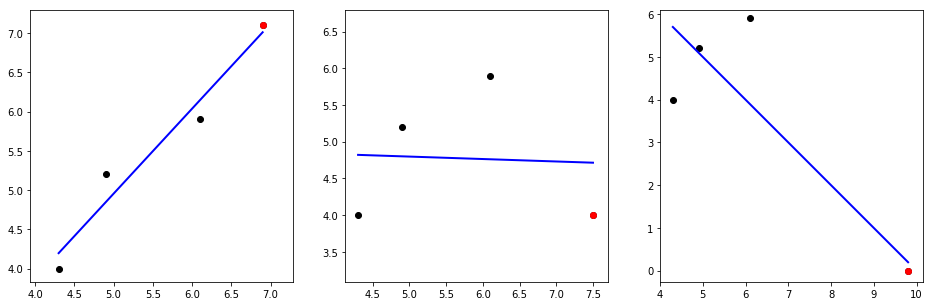
\includegraphics[width=11cm]{outlier_regression}
      % \label{figure:outlier:hyperplane}
  \end{figure}
  Change of the regression hyperplane given by coefficients estimated with OLS method when one of the four observations (highlighted with red color) starts to deviate from the linear pattern.
\end{frame}


%%%%%%%% FRAME 5  %%%%%%%%%%%%%%%
\begin{frame}{Robust statistics}
  \begin{itemize}
    \item Assumptions about the data are usually not fulfilled
    \item It is necessary to introduce methods that can deal with outliers
    \item Robust alternatives to OLS:
    \begin{itemize}
      \item Least trimmed squares (LTS)
      \item Weighted least squares (WLS)
      \item Least Median squares (LMS)
      \item M-estimators
      \item \dots
     \end{itemize}
   \end{itemize}
\end{frame}

%%%%%%%%%%%%%%%%%%%%%%%%%%%%%%%%%%%%%%%%%%%%%%%%%%%%%%%%%%%%%%%
%%%%%%%%%%%%%%%%%%% SECTION - OBJECTIVE %%%%%%%%%%%%%%%%%%%%%%%
%%%%%%%%%%%%%%%%%%%%%%%%%%%%%%%%%%%%%%%%%%%%%%%%%%%%%%%%%%%%%%%
\section{Objective}
\setcounter{subsection}{1}

%%%%%%%%%%%%% FRAME 1 %%%%%%%%%%%%%%%%%
\begin{frame}{Objective}
\begin{itemize}
\item  Describe robust regression methods and give a detail description of the LTS method
\item Survey known algorithms for computing the LTS estimate
\item Create a generator of data sets enabling to set various parameters like data size, contamination, contamination distribution etc.
\item Implement selected algorithms use these data sets to compare their performance
\end{itemize}
\end{frame}




%%%%%%%%%%%%%%%%%%%%%%%%%%%%%%%%%%%%%%%%%%%%%%%%%%%%%%%%%%%%%%%
%%%%%%%%%%%%%%%%%%% SECTION - LTS %%%%%%%%%%%%%%%%%%%%%%%%%%%%%
%%%%%%%%%%%%%%%%%%%%%%%%%%%%%%%%%%%%%%%%%%%%%%%%%%%%%%%%%%%%%%%
\section{Least trimmed squares}
\setcounter{subsection}{1}

%%%%%%%%%%%% FRAME 1 %%%%%%%%%%%%%%%
\begin{frame}{LTS}
\begin{itemize}
  \item Use only subset of the observations
  \item Select $h$ observations out of $n$ with smallest squared residuals from the regression hyperplane
\end{itemize}

\begin{equation*}  
        \of^{(LTS,h, n)}(\vec{w}) =  \sum\limits_{i=1}^h r_{i:n}^2(\vec{w})  
\end{equation*}
\end{frame}

%%%%%%%%%%%% FRAME 2 %%%%%%%%%%%%%%%
\begin{frame}{Problems with LTS objective function}

\begin{itemize}
  \item We do not know the hyperplane in advance
  \item We use sorted residuals
  \item Objective function is not differentiable and not convex
  \item Finding the exact solution is NP-hard
  \item {\color{red} Combinatorial optimization}
\end{itemize}    
\end{frame}

%%%%%%%%%%%% FRAME 3 %%%%%%%%%%%%%%%
\begin{frame}{Algorithms}

\begin{itemize}
    \item Exact algorithms
    \begin{itemize}
       \item BSA
       \item BAB
       \item BSABAB
    \end{itemize}    
\end{itemize}    

\begin{itemize}
  \item Probabilistic algorithms
  \begin{itemize}
    \item FAST-LTS
    \item FSA
    \item OEA
    \item MOEA
    \item MMEA
  \end{itemize}      
\end{itemize}    


\end{frame}


%%%%%%%%%%%%%%%%%%%%%%%%%%%%%%%%%%%%%%%%%%%%%%%%%%%%%%%%%%%%%%%
%%%%%%%%%%%%%%%%%%% SECTION - RESULTS %%%%%%%%%%%%%%%%%%%%%%%%%
%%%%%%%%%%%%%%%%%%%%%%%%%%%%%%%%%%%%%%%%%%%%%%%%%%%%%%%%%%%%%%%
\section{Results}
\setcounter{subsection}{1}

%%%%%%%%%%%% FRAME 1 %%%%%%%%%%%%%%%
\begin{frame}{Experiments}

\begin{itemize}
   \item Implementation
   \begin{itemize}
      \item All currently known algorithms
      \item Multiple combinations of those algorithms
      \item Some of our ideas of improvements of those algorithms
      \item Data set generator
   \end{itemize}       
   \item Experiments
   \begin{itemize}
      \item Quality and reliability of solutions
      \item Speed of the algorithms
   \end{itemize}       
\end{itemize}    
\end{frame}

%%%%%%%%%%%% FRAME 2 %%%%%%%%%%%%%%%
\begin{frame}{Experiments}
\begin{figure}[h]
    \centering
    % \missingfigure{Image visualizing  one C-step}
    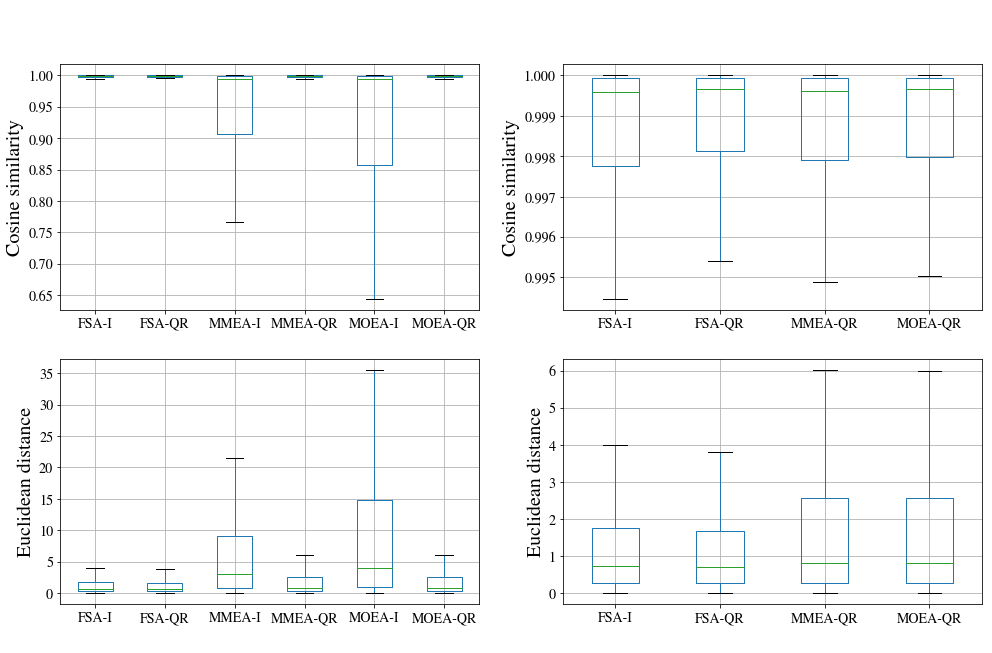
\includegraphics[width=11cm]{all_distances_feasible}
    
    % \label{all:distances}
\end{figure}
\end{frame}

%%%%%%%%%%%%%%%%%%%%%%%%%%%%%%%%%%%%%%%%%%%%%%%%%%%%%%%%%%%%%%%
%%%%%%%%%%%%%%%%% SECTION - CONCLUSION %%%%%%%%%%%%%%%%%%%%%%%%
%%%%%%%%%%%%%%%%%%%%%%%%%%%%%%%%%%%%%%%%%%%%%%%%%%%%%%%%%%%%%%%
\section{Conclusion}
\setcounter{subsection}{1}

%%%%%%%%%%%% FRAME 1 %%%%%%%%%%%%%%%
\begin{frame}{Conclusion}
  \begin{itemize}
    \item[\checkmark]  Describe robust regression methods and give a detail description of the LTS method
    \item[\checkmark] Survey known algorithms for computing the LTS estimate
    \item[\checkmark] Create a generator of data sets enabling to set various parameters like data size, contamination, contamination distribution etc.
    \item[\checkmark] Implement selected algorithms and use these data sets to compare their performance
  \end{itemize}      
\end{frame}


%%%%%%%%%%%% FRAME 5 %%%%%%%%%%%%%%%
\begin{frame}{Conclusion}
  \begin{center}
    Thank you for your attention.
  \end{center}
\end{frame}

%%%%%%%%%%%% FRAME 2 %%%%%%%%%%%%%%%
\begin{frame}{Questions}
  \begin{itemize}
    \item Why some simulations were not performed?
  \end{itemize}      
\end{frame}
% Proč nebyly provedeny simulace pro některé kombinace parametrů (např. tabulky 3.1 a A.1-A.6)?


%%%%%%%%%%%% FRAME 3 %%%%%%%%%%%%%%%
\begin{frame}{Questions}
  \begin{itemize}
    \item Why FSA-QR significantly improves BAB algorithm but not the BSA algorithm?
  \end{itemize}      

  \begin{figure}[h]
    \centering
    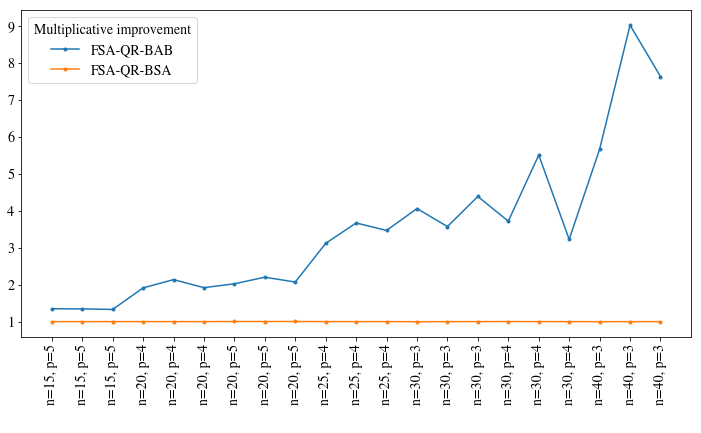
\includegraphics[width=9cm]{exact_improvement}
    % \label{figure:outlier:hyperplane}
  \end{figure}
\end{frame}
% Jaký je možný důvod, že FSA-QR varianta významně vylepší algoritmus BAB, ale ne BSA (tabulky A.4-A.6)?

%%%%%%%%%%%% FRAME 4 %%%%%%%%%%%%%%%
\begin{frame}{Questions}
  \begin{itemize}
    \item Why MMEA-QR results are different in tables A.1 a A.10 and  A.3 a A.12?
     (In some cases average time and L2 distance is up to two times worser.)
  \end{itemize}      
\end{frame}
% - Proč se od sebe liší výsledky pro algoritmus MMEA-QR v tabulkách A.1 a A.10, případně A.3 a A.12? V některých případech jsou průměrný čas a L2 vzdálenost až dvojnásobné.



%%%%%%%%%%%%%%%%%%%%%%%%%%%%%%%%%%%%%%%%%
%%%%%%%%% END DOCUMENT %%%%%%%%%%%%%%%%%%
%%%%%%%%%%%%%%%%%%%%%%%%%%%%%%%%%%%%%%%%%
% nebezelo to 100x l2 nomra muze hodne vystrelit a zamichat to fluktuace jso mouzne diky tomuto
% cas - 
% l2 norma nerobustni ale je to zvyk
\end{document}


